\documentclass{beamer}
\usetheme{Frankfurt}
\usepackage[utf8]{inputenc}
\usepackage{charter}
\usepackage{graphicx}
\usepackage{amsmath}
\usepackage{amssymb}
\usepackage{listings}
\usepackage{animate}
\usepackage{bm}
\usepackage{mathtools}
\usepackage{physics}
\usepackage{caption}
\usepackage{tikz}
\usepackage{tikz-cd}
\captionsetup[figure]{labelformat=empty}
\mathtoolsset{showonlyrefs}
\beamertemplatenavigationsymbolsempty

\let\vec\bm

\usepackage{tikzit}
\documentclass{beamer}
\usetheme{Frankfurt}
\usepackage[utf8]{inputenc}
\usepackage{charter}
\usepackage{graphicx}
\usepackage{amsmath}
\usepackage{amssymb}
\usepackage{listings}
\usepackage{animate}
\usepackage{bm}
\usepackage{mathtools}
\usepackage{physics}
\usepackage{caption}
\usepackage{tikz}
\usepackage{tikz-cd}
\captionsetup[figure]{labelformat=empty}
\mathtoolsset{showonlyrefs}
\beamertemplatenavigationsymbolsempty

\let\vec\bm

\usepackage{tikzit}
\documentclass{beamer}
\usetheme{Frankfurt}
\usepackage[utf8]{inputenc}
\usepackage{charter}
\usepackage{graphicx}
\usepackage{amsmath}
\usepackage{amssymb}
\usepackage{listings}
\usepackage{animate}
\usepackage{bm}
\usepackage{mathtools}
\usepackage{physics}
\usepackage{caption}
\usepackage{tikz}
\usepackage{tikz-cd}
\captionsetup[figure]{labelformat=empty}
\mathtoolsset{showonlyrefs}
\beamertemplatenavigationsymbolsempty

\let\vec\bm

\usepackage{tikzit}
\documentclass{beamer}
\usetheme{Frankfurt}
\usepackage[utf8]{inputenc}
\usepackage{charter}
\usepackage{graphicx}
\usepackage{amsmath}
\usepackage{amssymb}
\usepackage{listings}
\usepackage{animate}
\usepackage{bm}
\usepackage{mathtools}
\usepackage{physics}
\usepackage{caption}
\usepackage{tikz}
\usepackage{tikz-cd}
\captionsetup[figure]{labelformat=empty}
\mathtoolsset{showonlyrefs}
\beamertemplatenavigationsymbolsempty

\let\vec\bm

\usepackage{tikzit}
\input{main.tikzstyles}

\pgfdeclareimage[width=\paperwidth]{titlebackground}{Images/title-slide-background.png}
\setbeamerfont{subtitle}{size=\tiny}
\setbeamertemplate{endpage}{
	\begin{picture}(0,0)
		\scalebox{1.01}{
		\put(-28.5,-163){%
			\pgfuseimage{titlebackground}
		}
		}
		\put(0,-115){%
			\begin{minipage}[b][4.5cm][t]{0.5\textwidth}
				\color{white}
				\usebeamerfont{title}
				{\textbf{Thank Your} \\ \textbf{For You Attention !}}
			\end{minipage}
		}
	\end{picture}
}
\setbeamertemplate{title page}{
	\begin{picture}(0,0)
		\scalebox{1.01}{
			\put(-28.5,-163){%
				\pgfuseimage{titlebackground}
			}
		}
		\put(0,-60){%
			\begin{minipage}[b][4.5cm][t]{0.7\textwidth}
				\color{white}
				\usebeamerfont{title}
				{\inserttitle\\[0.9cm]}
				\usebeamerfont{subtitle}
				{\insertauthor\par}
				{\insertinstitute\\[0.3cm]}
				{\insertdate}
			\end{minipage}
		}
	\end{picture}
}


%% General slide formatting %%

\definecolor{oxfordblue}{RGB}{4,30,66}
\definecolor{oxfordred}{RGB}{207,48,42}

\pgfdeclareimage[width=0.9cm]{oxfordlogo}{Images/oxford-logo.png}
\pgfdeclareimage[width=1cm]{mathslogo}{Images/mathematics-logo.png}
\pgfdeclareimage[width=1.2cm]{ngslogo}{Images/ngs-logo.png}
\pgfdeclareimage[width=1.2cm]{petsclogo}{Images/petsc-logo.png}
\pgfdeclareimage[width=1.2cm]{firedrakelogo}{Images/firedrake-logo.png}

\setbeamertemplate{headline}
{%
	\begin{picture}(0,0)
		\put(314,-50){%
			\pgfuseimage{oxfordlogo}
		}
		\put(20,-55){%
			\rule{320pt}{0.4pt}
		}
	\end{picture}
}
\def\ngshead{
	\begin{picture}(0,0)
		\put(278,0){%
			\pgfuseimage{ngslogo}
		}
		\put(-8,-5){%
			\rule{325pt}{0.4pt}
		}
	\end{picture}
}
\def\petschead{
	\begin{picture}(0,0)
		\put(278,0){%
			\pgfuseimage{petsclogo}
		}
		\put(-8,-5){%
			\rule{325pt}{0.4pt}
		}
	\end{picture}
}
\def\firedrakehead{
	\begin{picture}(0,0)
		\put(278,0){%
			\pgfuseimage{firedrakelogo}
		}
		\put(-8,-5){%
			\rule{325pt}{0.4pt}
		}
	\end{picture}
}
\setbeamertemplate{frametitle}
{%
	\begin{picture}(0,0)
		\put(-8,-20){%
			\normalsize\textbf{\color{oxfordblue}\insertframetitle}
		}
		\put(-8,-32){%
			\normalsize\textbf{\color{oxfordblue}\insertframesubtitle}
		}
	\end{picture}
}

\setbeamertemplate{footline}
{%
	\begin{picture}(0,0)
		\put(20,30){%
			\rule{320pt}{0.4pt}
		}
		\put(20,14){%
			\pgfuseimage{mathslogo}
		}
		\put(100,14){%
			\color{oxfordblue}\insertshortdate
		}
		\put(160,14){%
			\color{oxfordblue}\insertshorttitle
		}
		\put(337,14){%
			\color{oxfordblue}\insertframenumber
		}
	\end{picture}%
}
\def\footer{
	\begin{picture}(0,0)
		\put(-308,-75){%
			\rule{325pt}{0.4pt}
		}
		\put(-308,-91){%
			\pgfuseimage{mathslogo}
		}
		\put(-228,-91){%
			\color{oxfordblue}\tiny\insertshortdate
		}
		\put(-168,-91){%
			\color{oxfordblue}\tiny\insertshorttitle
		}
		\put(9,-91){%
			\color{oxfordblue}\tiny\insertframenumber
		}
	\end{picture}
}

\setbeamercolor{block title}{bg=oxfordblue!30,fg=black}
\setbeamercolor{palette primary}{bg=oxfordblue,fg=white}

\definecolor{codegreen}{rgb}{0,0.6,0}
\definecolor{codegray}{rgb}{0.5,0.5,0.5}
\definecolor{codepurple}{rgb}{0.58,0,0.82}
\definecolor{backcolour}{rgb}{0.95,0.95,0.92}

\lstdefinestyle{mystyle}{
	%backgroundcolor=\color{backcolour},   
	commentstyle=\color{codegray},
	keywordstyle=\color{oxfordblue},
	numberstyle=\tiny\color{codegray},
	stringstyle=\color{codegreen},
	basicstyle=\ttfamily\footnotesize,
	breakatwhitespace=false,         
	breaklines=true,                 
	captionpos=b,                    
	keepspaces=true,                 
	numbers=left,                    
	numbersep=5pt,                  
	showspaces=false,                
	showstringspaces=false,
	showtabs=false,                  
	tabsize=2
}
\AtBeginSection[]{
  \begin{frame}
  \vfill
  \centering
  \begin{beamercolorbox}[sep=8pt,center,shadow=true,rounded=true]{title}
    \usebeamerfont{title}\insertsectionhead\par%
  \end{beamercolorbox}
  \vfill
  \end{frame}
}

\lstset{style=mystyle}

%% Information (author, title, etc.) %%
\title[ngsPETSc]{ngsPETSc: NETGEN meets PETSc} % short title for footer
\author%
{%
	\sc{P.~E.~Farrell}*, \sc{S.~Zampini$\dag$}, \underline{\sc{U.~Zerbinati}}*\\
}
\institute%
{%
	* \textit{Mathematical Institute}\\
	\;\textit{University of Oxford}\\
	$\newline$
	$\dag$ \textit{Extreme Computing Research Center}\\
	\;\textit{King Abdullah University of Science and Technology}\\	
}

\date[\textbf{PETSc 24}]{PETSc User Meeting, 23rd of May 2024, Cologne} % short date for footer



%% Content of slides %%

\begin{document}
	\begin{frame}[plain]
		\titlepage
	\end{frame}
	\begin{frame}{Overview}
		\begin{itemize}
			\item[\color{oxfordblue}$\blacktriangleright$]
			%\item[\color{oxfordblue}$\blacktriangleright$] Reynolds robust geometric multigrid on curved meshes.
			%\item[\color{oxfordblue}$\blacktriangleright$] Easy implementation:
		\end{itemize}
		\begin{minipage}{0.58\textwidth}
			All codes are available on Github:
			\texttt{https://github.com/UZerbinati/DD28}
		\end{minipage}
		\begin{minipage}{0.3\textwidth}
			\begin{figure}
				\centering
				\includegraphics[scale=0.2]{Figures/Github.png}
			\end{figure}
		\end{minipage}
	\end{frame}
	\begin{frame}[plain]
		\frametitle{Netgen/NGSolve}
		\ngshead
		$\newline$
		$\newline$
		$\newline$
		\textbf{Netgen} is an advancing front 2D/3D-mesh generator, with many interesting features.
		\begin{itemize}
			\item[\color{oxfordblue}$\blacktriangleright$] The geometry we intend to mesh can be described by \textbf{Constructive Solid Geometry} (CSG), in particular we can use \textbf{Opencascade} to describe our geometry.
			\item[\color{oxfordblue}$\blacktriangleright$] It is able to construct \textbf{isoparametric meshes} reppresentation, which conform to the geometry.
			\item[\color{oxfordblue}$\blacktriangleright$] A wide variety of mesh splits are available also for curved geometries, such as Alfeld splits and Powell-Sabin splits. 
			\item[\color{oxfordblue}$\blacktriangleright$] High flexibility in the mesh generation and mesh refinement.
		\end{itemize}
	\end{frame}
	\begin{frame}[plain]
		\frametitle{Netgen/NGSolve}
		\ngshead
		$\newline$
		$\newline$
		$\newline$
		\textbf{NGSolve} is a high-performance multiphysics finite element software with an extremely flexible Python interface.
		\begin{itemize}
			\item[\color{oxfordblue}$\blacktriangleright$] Wide range of finite elements available, including and not limited to hierarchical $H^1$ elements, $H(div)$ Raviart-Thomas and Brezzi-Douglas-Marini elements, and $H(curl)$ Nedelec elements.
			\item[\color{oxfordblue}$\blacktriangleright$] The variational formulation can be easily defined using an analogous language to the unified form language (UFL).
			\item[\color{oxfordblue}$\blacktriangleright$] Many extensions are available, including \textbf{ngsxfem} for unfitted finite element discretizations, \textbf{ngsTreffetz} for Treffetz methods and \textbf{ngsTents} for spacetime tents schemes.
		\end{itemize}
	\end{frame}
	\begin{frame}
		\frametitle{ngsPETSc -- NETGEN/NGSolve}
		$\newline$
		\textbf{ngsPETSc} is an interface between NETGEN/NGSolve and \textbf{PETSc}. In particular, \textbf{ngsPETSc} provides new capabilities to \textbf{NETGEN}/\textbf{NGSolve} such as:
		$\newline$
		\begin{itemize}
			\item[\color{oxfordblue}$\blacktriangleright$] Access to all linear solver capabilities of \textbf{KSP}.
			\item[\color{oxfordblue}$\blacktriangleright$] Access to all preconditioning capabilities of \textbf{PC}.
			\item[\color{oxfordblue}$\blacktriangleright$] Access to all non-linear solver capabilities of \textbf{SNES}.
			\item[\color{oxfordblue}$\blacktriangleright$] Access to all mesh refinement capabilities of \textbf{DMPLEX}.
		\end{itemize}
	\end{frame}
	\section{\textbf{PETSc KSP}}
	\begin{frame}[plain]
		\frametitle{An NGsolve Example}
		\ngshead
		$\newline$
		\lstinputlisting[language=Python, firstline=12, lastline=26]{../examples/ngs/ksp_poisson.py.rst}
	\end{frame}
	\begin{frame}[plain]
		\frametitle{PETSc KSP -- Direct solve with MUMPS }
		\ngshead
		$\newline$
		$\newline$
		\color{oxfordblue}$\blacktriangleright$ We can perform a direct solve using MUMPS.
		\begin{columns}[T]
			\begin{column}{0.7\textwidth}
				\lstinputlisting[language=Python, firstline=37, lastline=45]{../examples/ngs/ksp_poisson.py.rst}
			\end{column}
			\begin{column}{0.3\textwidth}
				\begin{figure}
					\centering
					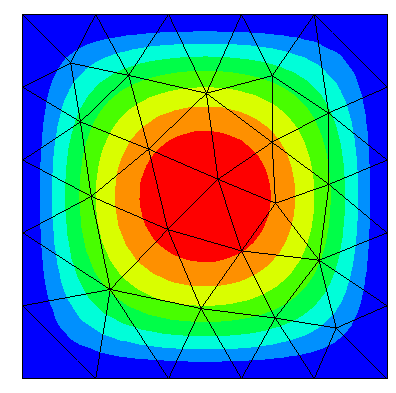
\includegraphics[scale=0.3]{../figures/mumps.png}
					\caption*{\tiny{Solution of Poisson problem computed with MUMPS}}
				\end{figure}
			\end{column}
		\end{columns}
	\end{frame}
	\begin{frame}[plain]
		\frametitle{PETSc KSP -- Iterative Jacobi method}
		\ngshead
		$\newline$
		$\newline$
		\color{oxfordblue}$\blacktriangleright$ We can use a wide variety of iterative solvers, for example, the Jacobi method, i.e.
		\begin{equation}
			x^{(k+1)} = D^{-1}(b - (A - D)x^{(k)}).
		\end{equation}
		\lstinputlisting[language=Python, firstline=52, lastline=58]{../examples/ngs/ksp_poisson.py.rst}
		$\newline$
		\color{oxfordblue}$\blacktriangleright$ Analogously we can implement the Gauss-Seidel method. 
	\end{frame}
	\begin{frame}[plain]
		\frametitle{PETSc KSP -- Geometric Algebraic MultiGrid (GAMG)}
		\ngshead
		$\newline$
		$\newline$
		$\newline$
		\color{oxfordblue}$\blacktriangleright$ Inside of a classical iterative method such as conjugate gradient, we can play with different preconditioners such as PETSc GAMG.
		$\newline$
		\lstinputlisting[language=Python, firstline=61, lastline=64]{../examples/ngs/ksp_poisson.py.rst}
		$\newline$
		\color{oxfordblue}$\blacktriangleright$ As we will see in a moment we have a wide variety of preconditioners available, such as: \textbf{Hypre (GAMG)}, \textbf{BDDC}, \textbf{...} 
	\end{frame}
	%\begin{frame}[plain]
	%	\firedrakehead
	%	$\newline$
	%	$\newline$
	%	\textbf{Firedrake} is an automated system for the solution of partial differential equations using the finite element method (FEM).
	%	$\newline$
	%	$\newline$
	%		\begin{itemize}
	%			\item[\color{oxfordblue}$\blacktriangleright$] Variational formulation can be easily defined using the \textbf{UFL} language.
	%			\item[\color{oxfordblue}$\blacktriangleright$] Wide class of finite elements are available, including $H(div)$, $H(curl)$, $H^1$ and $H^2$.
	%			\item[\color{oxfordblue}$\blacktriangleright$] Provides access to \textbf{PETSc} linear solvers and non-linear solvers.
	%		\end{itemize}
	%\end{frame}
	%\begin{frame}
	%	\frametitle{ngsPETSc -- Firedrake}
	%	$\newline$
	%	\textbf{ngsPETSc} provides new capabilities to \textbf{Firedrake} such as:
	%	$\newline$
	%	\begin{itemize}
	%		\item[\color{oxfordblue}$\blacktriangleright$] Access to all Netgen generated linear meshes and high order meshes.
	%		\item[\color{oxfordblue}$\blacktriangleright$] Splits for macro elements, such as Alfeld splits and Powell-Sabin splits (even on curved geometries).
	%		\item[\color{oxfordblue}$\blacktriangleright$] Adaptive mesh refinement capabilities, that conform to the geometry.
	%		\item[\color{oxfordblue}$\blacktriangleright$] High order mesh hierarchies for multigrid solvers. 
	%	\end{itemize}
	%\end{frame}
	%\begin{frame}
	%	\frametitle{Firedrake' 24}
	%	$\newline$
	%	Join us at the Firedrake user and developer workshop that will be held between 16-18 September 2024 at the University of Oxford.
	%\end{frame}
\end{document}


\pgfdeclareimage[width=\paperwidth]{titlebackground}{Images/title-slide-background.png}
\setbeamerfont{subtitle}{size=\tiny}
\setbeamertemplate{endpage}{
	\begin{picture}(0,0)
		\scalebox{1.01}{
		\put(-28.5,-163){%
			\pgfuseimage{titlebackground}
		}
		}
		\put(0,-115){%
			\begin{minipage}[b][4.5cm][t]{0.5\textwidth}
				\color{white}
				\usebeamerfont{title}
				{\textbf{Thank Your} \\ \textbf{For You Attention !}}
			\end{minipage}
		}
	\end{picture}
}
\setbeamertemplate{title page}{
	\begin{picture}(0,0)
		\scalebox{1.01}{
			\put(-28.5,-163){%
				\pgfuseimage{titlebackground}
			}
		}
		\put(0,-60){%
			\begin{minipage}[b][4.5cm][t]{0.7\textwidth}
				\color{white}
				\usebeamerfont{title}
				{\inserttitle\\[0.9cm]}
				\usebeamerfont{subtitle}
				{\insertauthor\par}
				{\insertinstitute\\[0.3cm]}
				{\insertdate}
			\end{minipage}
		}
	\end{picture}
}


%% General slide formatting %%

\definecolor{oxfordblue}{RGB}{4,30,66}
\definecolor{oxfordred}{RGB}{207,48,42}

\pgfdeclareimage[width=0.9cm]{oxfordlogo}{Images/oxford-logo.png}
\pgfdeclareimage[width=1cm]{mathslogo}{Images/mathematics-logo.png}
\pgfdeclareimage[width=1.2cm]{ngslogo}{Images/ngs-logo.png}
\pgfdeclareimage[width=1.2cm]{petsclogo}{Images/petsc-logo.png}
\pgfdeclareimage[width=1.2cm]{firedrakelogo}{Images/firedrake-logo.png}

\setbeamertemplate{headline}
{%
	\begin{picture}(0,0)
		\put(314,-50){%
			\pgfuseimage{oxfordlogo}
		}
		\put(20,-55){%
			\rule{320pt}{0.4pt}
		}
	\end{picture}
}
\def\ngshead{
	\begin{picture}(0,0)
		\put(278,0){%
			\pgfuseimage{ngslogo}
		}
		\put(-8,-5){%
			\rule{325pt}{0.4pt}
		}
	\end{picture}
}
\def\petschead{
	\begin{picture}(0,0)
		\put(278,0){%
			\pgfuseimage{petsclogo}
		}
		\put(-8,-5){%
			\rule{325pt}{0.4pt}
		}
	\end{picture}
}
\def\firedrakehead{
	\begin{picture}(0,0)
		\put(278,0){%
			\pgfuseimage{firedrakelogo}
		}
		\put(-8,-5){%
			\rule{325pt}{0.4pt}
		}
	\end{picture}
}
\setbeamertemplate{frametitle}
{%
	\begin{picture}(0,0)
		\put(-8,-20){%
			\normalsize\textbf{\color{oxfordblue}\insertframetitle}
		}
		\put(-8,-32){%
			\normalsize\textbf{\color{oxfordblue}\insertframesubtitle}
		}
	\end{picture}
}

\setbeamertemplate{footline}
{%
	\begin{picture}(0,0)
		\put(20,30){%
			\rule{320pt}{0.4pt}
		}
		\put(20,14){%
			\pgfuseimage{mathslogo}
		}
		\put(100,14){%
			\color{oxfordblue}\insertshortdate
		}
		\put(160,14){%
			\color{oxfordblue}\insertshorttitle
		}
		\put(337,14){%
			\color{oxfordblue}\insertframenumber
		}
	\end{picture}%
}
\def\footer{
	\begin{picture}(0,0)
		\put(-308,-75){%
			\rule{325pt}{0.4pt}
		}
		\put(-308,-91){%
			\pgfuseimage{mathslogo}
		}
		\put(-228,-91){%
			\color{oxfordblue}\tiny\insertshortdate
		}
		\put(-168,-91){%
			\color{oxfordblue}\tiny\insertshorttitle
		}
		\put(9,-91){%
			\color{oxfordblue}\tiny\insertframenumber
		}
	\end{picture}
}

\setbeamercolor{block title}{bg=oxfordblue!30,fg=black}
\setbeamercolor{palette primary}{bg=oxfordblue,fg=white}

\definecolor{codegreen}{rgb}{0,0.6,0}
\definecolor{codegray}{rgb}{0.5,0.5,0.5}
\definecolor{codepurple}{rgb}{0.58,0,0.82}
\definecolor{backcolour}{rgb}{0.95,0.95,0.92}

\lstdefinestyle{mystyle}{
	%backgroundcolor=\color{backcolour},   
	commentstyle=\color{codegray},
	keywordstyle=\color{oxfordblue},
	numberstyle=\tiny\color{codegray},
	stringstyle=\color{codegreen},
	basicstyle=\ttfamily\footnotesize,
	breakatwhitespace=false,         
	breaklines=true,                 
	captionpos=b,                    
	keepspaces=true,                 
	numbers=left,                    
	numbersep=5pt,                  
	showspaces=false,                
	showstringspaces=false,
	showtabs=false,                  
	tabsize=2
}
\AtBeginSection[]{
  \begin{frame}
  \vfill
  \centering
  \begin{beamercolorbox}[sep=8pt,center,shadow=true,rounded=true]{title}
    \usebeamerfont{title}\insertsectionhead\par%
  \end{beamercolorbox}
  \vfill
  \end{frame}
}

\lstset{style=mystyle}

%% Information (author, title, etc.) %%
\title[ngsPETSc]{ngsPETSc: NETGEN meets PETSc} % short title for footer
\author%
{%
	\sc{P.~E.~Farrell}*, \sc{S.~Zampini$\dag$}, \underline{\sc{U.~Zerbinati}}*\\
}
\institute%
{%
	* \textit{Mathematical Institute}\\
	\;\textit{University of Oxford}\\
	$\newline$
	$\dag$ \textit{Extreme Computing Research Center}\\
	\;\textit{King Abdullah University of Science and Technology}\\	
}

\date[\textbf{PETSc 24}]{PETSc User Meeting, 23rd of May 2024, Cologne} % short date for footer



%% Content of slides %%

\begin{document}
	\begin{frame}[plain]
		\titlepage
	\end{frame}
	\begin{frame}{Overview}
		\begin{itemize}
			\item[\color{oxfordblue}$\blacktriangleright$]
			%\item[\color{oxfordblue}$\blacktriangleright$] Reynolds robust geometric multigrid on curved meshes.
			%\item[\color{oxfordblue}$\blacktriangleright$] Easy implementation:
		\end{itemize}
		\begin{minipage}{0.58\textwidth}
			All codes are available on Github:
			\texttt{https://github.com/UZerbinati/DD28}
		\end{minipage}
		\begin{minipage}{0.3\textwidth}
			\begin{figure}
				\centering
				\includegraphics[scale=0.2]{Figures/Github.png}
			\end{figure}
		\end{minipage}
	\end{frame}
	\begin{frame}[plain]
		\frametitle{Netgen/NGSolve}
		\ngshead
		$\newline$
		$\newline$
		$\newline$
		\textbf{Netgen} is an advancing front 2D/3D-mesh generator, with many interesting features.
		\begin{itemize}
			\item[\color{oxfordblue}$\blacktriangleright$] The geometry we intend to mesh can be described by \textbf{Constructive Solid Geometry} (CSG), in particular we can use \textbf{Opencascade} to describe our geometry.
			\item[\color{oxfordblue}$\blacktriangleright$] It is able to construct \textbf{isoparametric meshes} reppresentation, which conform to the geometry.
			\item[\color{oxfordblue}$\blacktriangleright$] A wide variety of mesh splits are available also for curved geometries, such as Alfeld splits and Powell-Sabin splits. 
			\item[\color{oxfordblue}$\blacktriangleright$] High flexibility in the mesh generation and mesh refinement.
		\end{itemize}
	\end{frame}
	\begin{frame}[plain]
		\frametitle{Netgen/NGSolve}
		\ngshead
		$\newline$
		$\newline$
		$\newline$
		\textbf{NGSolve} is a high-performance multiphysics finite element software with an extremely flexible Python interface.
		\begin{itemize}
			\item[\color{oxfordblue}$\blacktriangleright$] Wide range of finite elements available, including and not limited to hierarchical $H^1$ elements, $H(div)$ Raviart-Thomas and Brezzi-Douglas-Marini elements, and $H(curl)$ Nedelec elements.
			\item[\color{oxfordblue}$\blacktriangleright$] The variational formulation can be easily defined using an analogous language to the unified form language (UFL).
			\item[\color{oxfordblue}$\blacktriangleright$] Many extensions are available, including \textbf{ngsxfem} for unfitted finite element discretizations, \textbf{ngsTreffetz} for Treffetz methods and \textbf{ngsTents} for spacetime tents schemes.
		\end{itemize}
	\end{frame}
	\begin{frame}
		\frametitle{ngsPETSc -- NETGEN/NGSolve}
		$\newline$
		\textbf{ngsPETSc} is an interface between NETGEN/NGSolve and \textbf{PETSc}. In particular, \textbf{ngsPETSc} provides new capabilities to \textbf{NETGEN}/\textbf{NGSolve} such as:
		$\newline$
		\begin{itemize}
			\item[\color{oxfordblue}$\blacktriangleright$] Access to all linear solver capabilities of \textbf{KSP}.
			\item[\color{oxfordblue}$\blacktriangleright$] Access to all preconditioning capabilities of \textbf{PC}.
			\item[\color{oxfordblue}$\blacktriangleright$] Access to all non-linear solver capabilities of \textbf{SNES}.
			\item[\color{oxfordblue}$\blacktriangleright$] Access to all mesh refinement capabilities of \textbf{DMPLEX}.
		\end{itemize}
	\end{frame}
	\section{\textbf{PETSc KSP}}
	\begin{frame}[plain]
		\frametitle{An NGsolve Example}
		\ngshead
		$\newline$
		\lstinputlisting[language=Python, firstline=12, lastline=26]{../examples/ngs/ksp_poisson.py.rst}
	\end{frame}
	\begin{frame}[plain]
		\frametitle{PETSc KSP -- Direct solve with MUMPS }
		\ngshead
		$\newline$
		$\newline$
		\color{oxfordblue}$\blacktriangleright$ We can perform a direct solve using MUMPS.
		\begin{columns}[T]
			\begin{column}{0.7\textwidth}
				\lstinputlisting[language=Python, firstline=37, lastline=45]{../examples/ngs/ksp_poisson.py.rst}
			\end{column}
			\begin{column}{0.3\textwidth}
				\begin{figure}
					\centering
					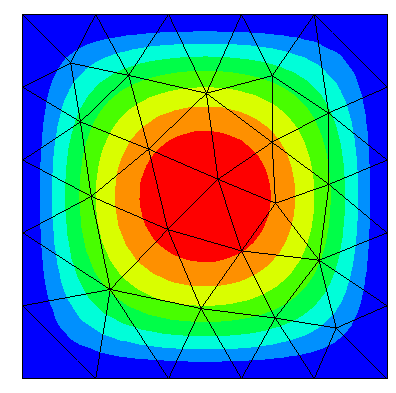
\includegraphics[scale=0.3]{../figures/mumps.png}
					\caption*{\tiny{Solution of Poisson problem computed with MUMPS}}
				\end{figure}
			\end{column}
		\end{columns}
	\end{frame}
	\begin{frame}[plain]
		\frametitle{PETSc KSP -- Iterative Jacobi method}
		\ngshead
		$\newline$
		$\newline$
		\color{oxfordblue}$\blacktriangleright$ We can use a wide variety of iterative solvers, for example, the Jacobi method, i.e.
		\begin{equation}
			x^{(k+1)} = D^{-1}(b - (A - D)x^{(k)}).
		\end{equation}
		\lstinputlisting[language=Python, firstline=52, lastline=58]{../examples/ngs/ksp_poisson.py.rst}
		$\newline$
		\color{oxfordblue}$\blacktriangleright$ Analogously we can implement the Gauss-Seidel method. 
	\end{frame}
	\begin{frame}[plain]
		\frametitle{PETSc KSP -- Geometric Algebraic MultiGrid (GAMG)}
		\ngshead
		$\newline$
		$\newline$
		$\newline$
		\color{oxfordblue}$\blacktriangleright$ Inside of a classical iterative method such as conjugate gradient, we can play with different preconditioners such as PETSc GAMG.
		$\newline$
		\lstinputlisting[language=Python, firstline=61, lastline=64]{../examples/ngs/ksp_poisson.py.rst}
		$\newline$
		\color{oxfordblue}$\blacktriangleright$ As we will see in a moment we have a wide variety of preconditioners available, such as: \textbf{Hypre (GAMG)}, \textbf{BDDC}, \textbf{...} 
	\end{frame}
	%\begin{frame}[plain]
	%	\firedrakehead
	%	$\newline$
	%	$\newline$
	%	\textbf{Firedrake} is an automated system for the solution of partial differential equations using the finite element method (FEM).
	%	$\newline$
	%	$\newline$
	%		\begin{itemize}
	%			\item[\color{oxfordblue}$\blacktriangleright$] Variational formulation can be easily defined using the \textbf{UFL} language.
	%			\item[\color{oxfordblue}$\blacktriangleright$] Wide class of finite elements are available, including $H(div)$, $H(curl)$, $H^1$ and $H^2$.
	%			\item[\color{oxfordblue}$\blacktriangleright$] Provides access to \textbf{PETSc} linear solvers and non-linear solvers.
	%		\end{itemize}
	%\end{frame}
	%\begin{frame}
	%	\frametitle{ngsPETSc -- Firedrake}
	%	$\newline$
	%	\textbf{ngsPETSc} provides new capabilities to \textbf{Firedrake} such as:
	%	$\newline$
	%	\begin{itemize}
	%		\item[\color{oxfordblue}$\blacktriangleright$] Access to all Netgen generated linear meshes and high order meshes.
	%		\item[\color{oxfordblue}$\blacktriangleright$] Splits for macro elements, such as Alfeld splits and Powell-Sabin splits (even on curved geometries).
	%		\item[\color{oxfordblue}$\blacktriangleright$] Adaptive mesh refinement capabilities, that conform to the geometry.
	%		\item[\color{oxfordblue}$\blacktriangleright$] High order mesh hierarchies for multigrid solvers. 
	%	\end{itemize}
	%\end{frame}
	%\begin{frame}
	%	\frametitle{Firedrake' 24}
	%	$\newline$
	%	Join us at the Firedrake user and developer workshop that will be held between 16-18 September 2024 at the University of Oxford.
	%\end{frame}
\end{document}


\pgfdeclareimage[width=\paperwidth]{titlebackground}{Images/title-slide-background.png}
\setbeamerfont{subtitle}{size=\tiny}
\setbeamertemplate{endpage}{
	\begin{picture}(0,0)
		\scalebox{1.01}{
		\put(-28.5,-163){%
			\pgfuseimage{titlebackground}
		}
		}
		\put(0,-115){%
			\begin{minipage}[b][4.5cm][t]{0.5\textwidth}
				\color{white}
				\usebeamerfont{title}
				{\textbf{Thank Your} \\ \textbf{For You Attention !}}
			\end{minipage}
		}
	\end{picture}
}
\setbeamertemplate{title page}{
	\begin{picture}(0,0)
		\scalebox{1.01}{
			\put(-28.5,-163){%
				\pgfuseimage{titlebackground}
			}
		}
		\put(0,-60){%
			\begin{minipage}[b][4.5cm][t]{0.7\textwidth}
				\color{white}
				\usebeamerfont{title}
				{\inserttitle\\[0.9cm]}
				\usebeamerfont{subtitle}
				{\insertauthor\par}
				{\insertinstitute\\[0.3cm]}
				{\insertdate}
			\end{minipage}
		}
	\end{picture}
}


%% General slide formatting %%

\definecolor{oxfordblue}{RGB}{4,30,66}
\definecolor{oxfordred}{RGB}{207,48,42}

\pgfdeclareimage[width=0.9cm]{oxfordlogo}{Images/oxford-logo.png}
\pgfdeclareimage[width=1cm]{mathslogo}{Images/mathematics-logo.png}
\pgfdeclareimage[width=1.2cm]{ngslogo}{Images/ngs-logo.png}
\pgfdeclareimage[width=1.2cm]{petsclogo}{Images/petsc-logo.png}
\pgfdeclareimage[width=1.2cm]{firedrakelogo}{Images/firedrake-logo.png}

\setbeamertemplate{headline}
{%
	\begin{picture}(0,0)
		\put(314,-50){%
			\pgfuseimage{oxfordlogo}
		}
		\put(20,-55){%
			\rule{320pt}{0.4pt}
		}
	\end{picture}
}
\def\ngshead{
	\begin{picture}(0,0)
		\put(278,0){%
			\pgfuseimage{ngslogo}
		}
		\put(-8,-5){%
			\rule{325pt}{0.4pt}
		}
	\end{picture}
}
\def\petschead{
	\begin{picture}(0,0)
		\put(278,0){%
			\pgfuseimage{petsclogo}
		}
		\put(-8,-5){%
			\rule{325pt}{0.4pt}
		}
	\end{picture}
}
\def\firedrakehead{
	\begin{picture}(0,0)
		\put(278,0){%
			\pgfuseimage{firedrakelogo}
		}
		\put(-8,-5){%
			\rule{325pt}{0.4pt}
		}
	\end{picture}
}
\setbeamertemplate{frametitle}
{%
	\begin{picture}(0,0)
		\put(-8,-20){%
			\normalsize\textbf{\color{oxfordblue}\insertframetitle}
		}
		\put(-8,-32){%
			\normalsize\textbf{\color{oxfordblue}\insertframesubtitle}
		}
	\end{picture}
}

\setbeamertemplate{footline}
{%
	\begin{picture}(0,0)
		\put(20,30){%
			\rule{320pt}{0.4pt}
		}
		\put(20,14){%
			\pgfuseimage{mathslogo}
		}
		\put(100,14){%
			\color{oxfordblue}\insertshortdate
		}
		\put(160,14){%
			\color{oxfordblue}\insertshorttitle
		}
		\put(337,14){%
			\color{oxfordblue}\insertframenumber
		}
	\end{picture}%
}
\def\footer{
	\begin{picture}(0,0)
		\put(-308,-75){%
			\rule{325pt}{0.4pt}
		}
		\put(-308,-91){%
			\pgfuseimage{mathslogo}
		}
		\put(-228,-91){%
			\color{oxfordblue}\tiny\insertshortdate
		}
		\put(-168,-91){%
			\color{oxfordblue}\tiny\insertshorttitle
		}
		\put(9,-91){%
			\color{oxfordblue}\tiny\insertframenumber
		}
	\end{picture}
}

\setbeamercolor{block title}{bg=oxfordblue!30,fg=black}
\setbeamercolor{palette primary}{bg=oxfordblue,fg=white}

\definecolor{codegreen}{rgb}{0,0.6,0}
\definecolor{codegray}{rgb}{0.5,0.5,0.5}
\definecolor{codepurple}{rgb}{0.58,0,0.82}
\definecolor{backcolour}{rgb}{0.95,0.95,0.92}

\lstdefinestyle{mystyle}{
	%backgroundcolor=\color{backcolour},   
	commentstyle=\color{codegray},
	keywordstyle=\color{oxfordblue},
	numberstyle=\tiny\color{codegray},
	stringstyle=\color{codegreen},
	basicstyle=\ttfamily\footnotesize,
	breakatwhitespace=false,         
	breaklines=true,                 
	captionpos=b,                    
	keepspaces=true,                 
	numbers=left,                    
	numbersep=5pt,                  
	showspaces=false,                
	showstringspaces=false,
	showtabs=false,                  
	tabsize=2
}
\AtBeginSection[]{
  \begin{frame}
  \vfill
  \centering
  \begin{beamercolorbox}[sep=8pt,center,shadow=true,rounded=true]{title}
    \usebeamerfont{title}\insertsectionhead\par%
  \end{beamercolorbox}
  \vfill
  \end{frame}
}

\lstset{style=mystyle}

%% Information (author, title, etc.) %%
\title[ngsPETSc]{ngsPETSc: NETGEN meets PETSc} % short title for footer
\author%
{%
	\sc{P.~E.~Farrell}*, \sc{S.~Zampini$\dag$}, \underline{\sc{U.~Zerbinati}}*\\
}
\institute%
{%
	* \textit{Mathematical Institute}\\
	\;\textit{University of Oxford}\\
	$\newline$
	$\dag$ \textit{Extreme Computing Research Center}\\
	\;\textit{King Abdullah University of Science and Technology}\\	
}

\date[\textbf{PETSc 24}]{PETSc User Meeting, 23rd of May 2024, Cologne} % short date for footer



%% Content of slides %%

\begin{document}
	\begin{frame}[plain]
		\titlepage
	\end{frame}
	\begin{frame}{Overview}
		\begin{itemize}
			\item[\color{oxfordblue}$\blacktriangleright$]
			%\item[\color{oxfordblue}$\blacktriangleright$] Reynolds robust geometric multigrid on curved meshes.
			%\item[\color{oxfordblue}$\blacktriangleright$] Easy implementation:
		\end{itemize}
		\begin{minipage}{0.58\textwidth}
			All codes are available on Github:
			\texttt{https://github.com/UZerbinati/DD28}
		\end{minipage}
		\begin{minipage}{0.3\textwidth}
			\begin{figure}
				\centering
				\includegraphics[scale=0.2]{Figures/Github.png}
			\end{figure}
		\end{minipage}
	\end{frame}
	\begin{frame}[plain]
		\frametitle{Netgen/NGSolve}
		\ngshead
		$\newline$
		$\newline$
		$\newline$
		\textbf{Netgen} is an advancing front 2D/3D-mesh generator, with many interesting features.
		\begin{itemize}
			\item[\color{oxfordblue}$\blacktriangleright$] The geometry we intend to mesh can be described by \textbf{Constructive Solid Geometry} (CSG), in particular we can use \textbf{Opencascade} to describe our geometry.
			\item[\color{oxfordblue}$\blacktriangleright$] It is able to construct \textbf{isoparametric meshes} reppresentation, which conform to the geometry.
			\item[\color{oxfordblue}$\blacktriangleright$] A wide variety of mesh splits are available also for curved geometries, such as Alfeld splits and Powell-Sabin splits. 
			\item[\color{oxfordblue}$\blacktriangleright$] High flexibility in the mesh generation and mesh refinement.
		\end{itemize}
	\end{frame}
	\begin{frame}[plain]
		\frametitle{Netgen/NGSolve}
		\ngshead
		$\newline$
		$\newline$
		$\newline$
		\textbf{NGSolve} is a high-performance multiphysics finite element software with an extremely flexible Python interface.
		\begin{itemize}
			\item[\color{oxfordblue}$\blacktriangleright$] Wide range of finite elements available, including and not limited to hierarchical $H^1$ elements, $H(div)$ Raviart-Thomas and Brezzi-Douglas-Marini elements, and $H(curl)$ Nedelec elements.
			\item[\color{oxfordblue}$\blacktriangleright$] The variational formulation can be easily defined using an analogous language to the unified form language (UFL).
			\item[\color{oxfordblue}$\blacktriangleright$] Many extensions are available, including \textbf{ngsxfem} for unfitted finite element discretizations, \textbf{ngsTreffetz} for Treffetz methods and \textbf{ngsTents} for spacetime tents schemes.
		\end{itemize}
	\end{frame}
	\begin{frame}
		\frametitle{ngsPETSc -- NETGEN/NGSolve}
		$\newline$
		\textbf{ngsPETSc} is an interface between NETGEN/NGSolve and \textbf{PETSc}. In particular, \textbf{ngsPETSc} provides new capabilities to \textbf{NETGEN}/\textbf{NGSolve} such as:
		$\newline$
		\begin{itemize}
			\item[\color{oxfordblue}$\blacktriangleright$] Access to all linear solver capabilities of \textbf{KSP}.
			\item[\color{oxfordblue}$\blacktriangleright$] Access to all preconditioning capabilities of \textbf{PC}.
			\item[\color{oxfordblue}$\blacktriangleright$] Access to all non-linear solver capabilities of \textbf{SNES}.
			\item[\color{oxfordblue}$\blacktriangleright$] Access to all mesh refinement capabilities of \textbf{DMPLEX}.
		\end{itemize}
	\end{frame}
	\section{\textbf{PETSc KSP}}
	\begin{frame}[plain]
		\frametitle{An NGsolve Example}
		\ngshead
		$\newline$
		\lstinputlisting[language=Python, firstline=12, lastline=26]{../examples/ngs/ksp_poisson.py.rst}
	\end{frame}
	\begin{frame}[plain]
		\frametitle{PETSc KSP -- Direct solve with MUMPS }
		\ngshead
		$\newline$
		$\newline$
		\color{oxfordblue}$\blacktriangleright$ We can perform a direct solve using MUMPS.
		\begin{columns}[T]
			\begin{column}{0.7\textwidth}
				\lstinputlisting[language=Python, firstline=37, lastline=45]{../examples/ngs/ksp_poisson.py.rst}
			\end{column}
			\begin{column}{0.3\textwidth}
				\begin{figure}
					\centering
					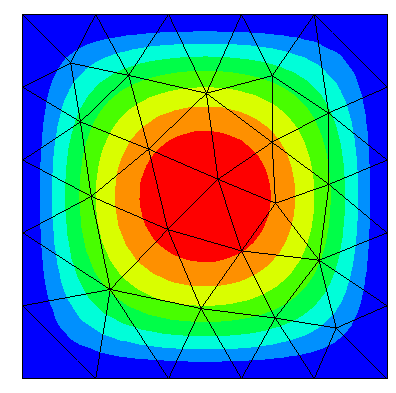
\includegraphics[scale=0.3]{../figures/mumps.png}
					\caption*{\tiny{Solution of Poisson problem computed with MUMPS}}
				\end{figure}
			\end{column}
		\end{columns}
	\end{frame}
	\begin{frame}[plain]
		\frametitle{PETSc KSP -- Iterative Jacobi method}
		\ngshead
		$\newline$
		$\newline$
		\color{oxfordblue}$\blacktriangleright$ We can use a wide variety of iterative solvers, for example, the Jacobi method, i.e.
		\begin{equation}
			x^{(k+1)} = D^{-1}(b - (A - D)x^{(k)}).
		\end{equation}
		\lstinputlisting[language=Python, firstline=52, lastline=58]{../examples/ngs/ksp_poisson.py.rst}
		$\newline$
		\color{oxfordblue}$\blacktriangleright$ Analogously we can implement the Gauss-Seidel method. 
	\end{frame}
	\begin{frame}[plain]
		\frametitle{PETSc KSP -- Geometric Algebraic MultiGrid (GAMG)}
		\ngshead
		$\newline$
		$\newline$
		$\newline$
		\color{oxfordblue}$\blacktriangleright$ Inside of a classical iterative method such as conjugate gradient, we can play with different preconditioners such as PETSc GAMG.
		$\newline$
		\lstinputlisting[language=Python, firstline=61, lastline=64]{../examples/ngs/ksp_poisson.py.rst}
		$\newline$
		\color{oxfordblue}$\blacktriangleright$ As we will see in a moment we have a wide variety of preconditioners available, such as: \textbf{Hypre (GAMG)}, \textbf{BDDC}, \textbf{...} 
	\end{frame}
	%\begin{frame}[plain]
	%	\firedrakehead
	%	$\newline$
	%	$\newline$
	%	\textbf{Firedrake} is an automated system for the solution of partial differential equations using the finite element method (FEM).
	%	$\newline$
	%	$\newline$
	%		\begin{itemize}
	%			\item[\color{oxfordblue}$\blacktriangleright$] Variational formulation can be easily defined using the \textbf{UFL} language.
	%			\item[\color{oxfordblue}$\blacktriangleright$] Wide class of finite elements are available, including $H(div)$, $H(curl)$, $H^1$ and $H^2$.
	%			\item[\color{oxfordblue}$\blacktriangleright$] Provides access to \textbf{PETSc} linear solvers and non-linear solvers.
	%		\end{itemize}
	%\end{frame}
	%\begin{frame}
	%	\frametitle{ngsPETSc -- Firedrake}
	%	$\newline$
	%	\textbf{ngsPETSc} provides new capabilities to \textbf{Firedrake} such as:
	%	$\newline$
	%	\begin{itemize}
	%		\item[\color{oxfordblue}$\blacktriangleright$] Access to all Netgen generated linear meshes and high order meshes.
	%		\item[\color{oxfordblue}$\blacktriangleright$] Splits for macro elements, such as Alfeld splits and Powell-Sabin splits (even on curved geometries).
	%		\item[\color{oxfordblue}$\blacktriangleright$] Adaptive mesh refinement capabilities, that conform to the geometry.
	%		\item[\color{oxfordblue}$\blacktriangleright$] High order mesh hierarchies for multigrid solvers. 
	%	\end{itemize}
	%\end{frame}
	%\begin{frame}
	%	\frametitle{Firedrake' 24}
	%	$\newline$
	%	Join us at the Firedrake user and developer workshop that will be held between 16-18 September 2024 at the University of Oxford.
	%\end{frame}
\end{document}


\pgfdeclareimage[width=\paperwidth]{titlebackground}{Images/title-slide-background.png}
\setbeamerfont{subtitle}{size=\tiny}
\setbeamertemplate{endpage}{
	\begin{picture}(0,0)
		\scalebox{1.01}{
		\put(-28.5,-163){%
			\pgfuseimage{titlebackground}
		}
		}
		\put(0,-115){%
			\begin{minipage}[b][4.5cm][t]{0.5\textwidth}
				\color{white}
				\usebeamerfont{title}
				{\textbf{Thank Your} \\ \textbf{For You Attention !}}
			\end{minipage}
		}
	\end{picture}
}
\setbeamertemplate{title page}{
	\begin{picture}(0,0)
		\scalebox{1.01}{
			\put(-28.5,-163){%
				\pgfuseimage{titlebackground}
			}
		}
		\put(0,-60){%
			\begin{minipage}[b][4.5cm][t]{0.7\textwidth}
				\color{white}
				\usebeamerfont{title}
				{\inserttitle\\[0.9cm]}
				\usebeamerfont{subtitle}
				{\insertauthor\par}
				{\insertinstitute\\[0.3cm]}
				{\insertdate}
			\end{minipage}
		}
	\end{picture}
}


%% General slide formatting %%

\definecolor{oxfordblue}{RGB}{4,30,66}
\definecolor{oxfordred}{RGB}{207,48,42}

\pgfdeclareimage[width=0.9cm]{oxfordlogo}{Images/oxford-logo.png}
\pgfdeclareimage[width=1cm]{mathslogo}{Images/mathematics-logo.png}
\pgfdeclareimage[width=1.2cm]{ngslogo}{Images/ngs-logo.png}
\pgfdeclareimage[width=1.2cm]{petsclogo}{Images/petsc-logo.png}
\pgfdeclareimage[width=1.2cm]{firedrakelogo}{Images/firedrake-logo.png}

\setbeamertemplate{headline}
{%
	\begin{picture}(0,0)
		\put(314,-50){%
			\pgfuseimage{oxfordlogo}
		}
		\put(20,-55){%
			\rule{320pt}{0.4pt}
		}
	\end{picture}
}
\def\ngshead{
	\begin{picture}(0,0)
		\put(278,0){%
			\pgfuseimage{ngslogo}
		}
		\put(-8,-5){%
			\rule{325pt}{0.4pt}
		}
	\end{picture}
}
\def\petschead{
	\begin{picture}(0,0)
		\put(278,0){%
			\pgfuseimage{petsclogo}
		}
		\put(-8,-5){%
			\rule{325pt}{0.4pt}
		}
	\end{picture}
}
\def\firedrakehead{
	\begin{picture}(0,0)
		\put(278,0){%
			\pgfuseimage{firedrakelogo}
		}
		\put(-8,-5){%
			\rule{325pt}{0.4pt}
		}
	\end{picture}
}
\setbeamertemplate{frametitle}
{%
	\begin{picture}(0,0)
		\put(-8,-20){%
			\normalsize\textbf{\color{oxfordblue}\insertframetitle}
		}
		\put(-8,-32){%
			\normalsize\textbf{\color{oxfordblue}\insertframesubtitle}
		}
	\end{picture}
}

\setbeamertemplate{footline}
{%
	\begin{picture}(0,0)
		\put(20,30){%
			\rule{320pt}{0.4pt}
		}
		\put(20,14){%
			\pgfuseimage{mathslogo}
		}
		\put(100,14){%
			\color{oxfordblue}\insertshortdate
		}
		\put(160,14){%
			\color{oxfordblue}\insertshorttitle
		}
		\put(337,14){%
			\color{oxfordblue}\insertframenumber
		}
	\end{picture}%
}
\def\footer{
	\begin{picture}(0,0)
		\put(-308,-75){%
			\rule{325pt}{0.4pt}
		}
		\put(-308,-91){%
			\pgfuseimage{mathslogo}
		}
		\put(-228,-91){%
			\color{oxfordblue}\tiny\insertshortdate
		}
		\put(-168,-91){%
			\color{oxfordblue}\tiny\insertshorttitle
		}
		\put(9,-91){%
			\color{oxfordblue}\tiny\insertframenumber
		}
	\end{picture}
}

\setbeamercolor{block title}{bg=oxfordblue!30,fg=black}
\setbeamercolor{palette primary}{bg=oxfordblue,fg=white}

\definecolor{codegreen}{rgb}{0,0.6,0}
\definecolor{codegray}{rgb}{0.5,0.5,0.5}
\definecolor{codepurple}{rgb}{0.58,0,0.82}
\definecolor{backcolour}{rgb}{0.95,0.95,0.92}

\lstdefinestyle{mystyle}{
	%backgroundcolor=\color{backcolour},   
	commentstyle=\color{codegray},
	keywordstyle=\color{oxfordblue},
	numberstyle=\tiny\color{codegray},
	stringstyle=\color{codegreen},
	basicstyle=\ttfamily\footnotesize,
	breakatwhitespace=false,         
	breaklines=true,                 
	captionpos=b,                    
	keepspaces=true,                 
	numbers=left,                    
	numbersep=5pt,                  
	showspaces=false,                
	showstringspaces=false,
	showtabs=false,                  
	tabsize=2
}
\AtBeginSection[]{
  \begin{frame}
  \vfill
  \centering
  \begin{beamercolorbox}[sep=8pt,center,shadow=true,rounded=true]{title}
    \usebeamerfont{title}\insertsectionhead\par%
  \end{beamercolorbox}
  \vfill
  \end{frame}
}

\lstset{style=mystyle}

%% Information (author, title, etc.) %%
\title[ngsPETSc]{ngsPETSc: NETGEN meets PETSc} % short title for footer
\author%
{%
	\sc{P.~E.~Farrell}*, \sc{S.~Zampini$\dag$}, \underline{\sc{U.~Zerbinati}}*\\
}
\institute%
{%
	* \textit{Mathematical Institute}\\
	\;\textit{University of Oxford}\\
	$\newline$
	$\dag$ \textit{Extreme Computing Research Center}\\
	\;\textit{King Abdullah University of Science and Technology}\\	
}

\date[\textbf{PETSc 24}]{PETSc User Meeting, 23rd of May 2024, Cologne} % short date for footer



%% Content of slides %%

\begin{document}
	\begin{frame}[plain]
		\titlepage
	\end{frame}
	\begin{frame}{Overview}
		\begin{itemize}
			\item[\color{oxfordblue}$\blacktriangleright$]
			%\item[\color{oxfordblue}$\blacktriangleright$] Reynolds robust geometric multigrid on curved meshes.
			%\item[\color{oxfordblue}$\blacktriangleright$] Easy implementation:
		\end{itemize}
		\begin{minipage}{0.58\textwidth}
			All codes are available on Github:
			\texttt{https://github.com/UZerbinati/DD28}
		\end{minipage}
		\begin{minipage}{0.3\textwidth}
			\begin{figure}
				\centering
				\includegraphics[scale=0.2]{Figures/Github.png}
			\end{figure}
		\end{minipage}
	\end{frame}
	\begin{frame}[plain]
		\frametitle{Netgen/NGSolve}
		\ngshead
		$\newline$
		$\newline$
		$\newline$
		\textbf{Netgen} is an advancing front 2D/3D-mesh generator, with many interesting features.
		\begin{itemize}
			\item[\color{oxfordblue}$\blacktriangleright$] The geometry we intend to mesh can be described by \textbf{Constructive Solid Geometry} (CSG), in particular we can use \textbf{Opencascade} to describe our geometry.
			\item[\color{oxfordblue}$\blacktriangleright$] It is able to construct \textbf{isoparametric meshes} reppresentation, which conform to the geometry.
			\item[\color{oxfordblue}$\blacktriangleright$] A wide variety of mesh splits are available also for curved geometries, such as Alfeld splits and Powell-Sabin splits. 
			\item[\color{oxfordblue}$\blacktriangleright$] High flexibility in the mesh generation and mesh refinement.
		\end{itemize}
	\end{frame}
	\begin{frame}[plain]
		\frametitle{Netgen/NGSolve}
		\ngshead
		$\newline$
		$\newline$
		$\newline$
		\textbf{NGSolve} is a high-performance multiphysics finite element software with an extremely flexible Python interface.
		\begin{itemize}
			\item[\color{oxfordblue}$\blacktriangleright$] Wide range of finite elements available, including and not limited to hierarchical $H^1$ elements, $H(div)$ Raviart-Thomas and Brezzi-Douglas-Marini elements, and $H(curl)$ Nedelec elements.
			\item[\color{oxfordblue}$\blacktriangleright$] The variational formulation can be easily defined using an analogous language to the unified form language (UFL).
			\item[\color{oxfordblue}$\blacktriangleright$] Many extensions are available, including \textbf{ngsxfem} for unfitted finite element discretizations, \textbf{ngsTreffetz} for Treffetz methods and \textbf{ngsTents} for spacetime tents schemes.
		\end{itemize}
	\end{frame}
	\begin{frame}
		\frametitle{ngsPETSc -- NETGEN/NGSolve}
		$\newline$
		\textbf{ngsPETSc} is an interface between NETGEN/NGSolve and \textbf{PETSc}. In particular, \textbf{ngsPETSc} provides new capabilities to \textbf{NETGEN}/\textbf{NGSolve} such as:
		$\newline$
		\begin{itemize}
			\item[\color{oxfordblue}$\blacktriangleright$] Access to all linear solver capabilities of \textbf{KSP}.
			\item[\color{oxfordblue}$\blacktriangleright$] Access to all preconditioning capabilities of \textbf{PC}.
			\item[\color{oxfordblue}$\blacktriangleright$] Access to all non-linear solver capabilities of \textbf{SNES}.
			\item[\color{oxfordblue}$\blacktriangleright$] Access to all mesh refinement capabilities of \textbf{DMPLEX}.
		\end{itemize}
	\end{frame}
	\begin{frame}[plain]
		\frametitle{An NGsolve Example}
		\ngshead
		$\newline$
		\lstinputlisting[language=Python, firstline=12, lastline=26]{../examples/ngs/ksp_poisson.py.rst}
	\end{frame}
	\begin{frame}[plain]
		\frametitle{PETSc KSP -- MUMPS}
		\ngshead
		$\newline$
		\begin{columns}[T]
			\begin{column}{0.7\textwidth}
				\lstinputlisting[language=Python, firstline=37, lastline=42]{../examples/ngs/ksp_poisson.py.rst}
			\end{column}
			\begin{column}{0.3\textwidth}
				\begin{figure}
					\centering
					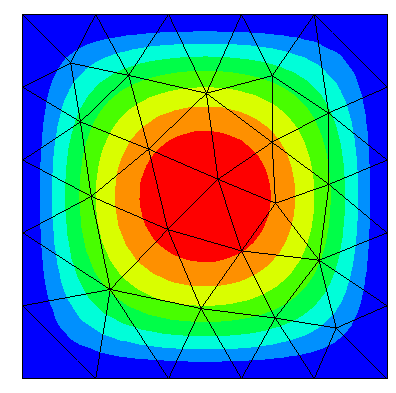
\includegraphics[scale=0.3]{../figures/mumps.png}
				\end{figure}
				
			\end{column}
		\end{columns}
	\end{frame}
	%\begin{frame}[plain]
	%	\firedrakehead
	%	$\newline$
	%	$\newline$
	%	\textbf{Firedrake} is an automated system for the solution of partial differential equations using the finite element method (FEM).
	%	$\newline$
	%	$\newline$
	%		\begin{itemize}
	%			\item[\color{oxfordblue}$\blacktriangleright$] Variational formulation can be easily defined using the \textbf{UFL} language.
	%			\item[\color{oxfordblue}$\blacktriangleright$] Wide class of finite elements are available, including $H(div)$, $H(curl)$, $H^1$ and $H^2$.
	%			\item[\color{oxfordblue}$\blacktriangleright$] Provides access to \textbf{PETSc} linear solvers and non-linear solvers.
	%		\end{itemize}
	%\end{frame}
	%\begin{frame}
	%	\frametitle{ngsPETSc -- Firedrake}
	%	$\newline$
	%	\textbf{ngsPETSc} provides new capabilities to \textbf{Firedrake} such as:
	%	$\newline$
	%	\begin{itemize}
	%		\item[\color{oxfordblue}$\blacktriangleright$] Access to all Netgen generated linear meshes and high order meshes.
	%		\item[\color{oxfordblue}$\blacktriangleright$] Splits for macro elements, such as Alfeld splits and Powell-Sabin splits (even on curved geometries).
	%		\item[\color{oxfordblue}$\blacktriangleright$] Adaptive mesh refinement capabilities, that conform to the geometry.
	%		\item[\color{oxfordblue}$\blacktriangleright$] High order mesh hierarchies for multigrid solvers. 
	%	\end{itemize}
	%\end{frame}
	%\begin{frame}
	%	\frametitle{Firedrake' 24}
	%	$\newline$
	%	Join us at the Firedrake user and developer workshop that will be held between 16-18 September 2024 at the University of Oxford.
	%\end{frame}
\end{document}
